\documentclass[11pt]{article}

%============================================================
% Packages
%============================================================
\usepackage[utf8]{inputenc}
\usepackage[T1]{fontenc}
\usepackage{amsmath,amssymb,amsfonts,mathtools}
\usepackage{bbm}
\usepackage{bm}
\usepackage{graphicx}
\usepackage{subcaption}
\usepackage{booktabs}
\usepackage{hyperref}
\usepackage{natbib}
\usepackage[margin=1in]{geometry}
\usepackage{tikz}
\usetikzlibrary{arrows.meta,positioning,calc}
\usepackage[ruled,vlined,linesnumbered]{algorithm2e}

\hypersetup{
    colorlinks=true,
    linkcolor=blue,
    citecolor=blue,
    urlcolor=blue
}

\graphicspath{{Figures/Figures_v3/}}

%============================================================
% Convenience macros
%============================================================
\newcommand{\Ret}{\mathrm{Ret}}
\newcommand{\eff}{\varepsilon}
\newcommand{\goth}[1]{\mathcal{#1}}   % gothic-script value of ending period with assets
\newcommand{\E}{\mathbb{E}}

\title{Search Smooths Discontinuities in\\ Discrete/Continuous Problems}

\author{
Christopher D.\ Carroll\thanks{Carroll: Department of Economics, Johns Hopkins University,
\url{http://econ.jhu.edu/people/ccarroll/}, \texttt{ccarroll@jhu.edu}.}\\
JHU
\and
Fedor Iskhakov\thanks{Iskhakov: ANU.}\\
ANU
\and
Shujaat Khan\thanks{Khan: IMF.}\\
JHU
}

\date{September 1, 2019}

%============================================================
\begin{document}
\maketitle

\begin{abstract}
When used to solve models with both discrete and continuous choices, the Endogenous
Gridpoint Method (EGM), in addition to finding the optimal solution, can also generate points
in the solution that are suboptimal. This paper shows that incorporating search into such
problems can smooth out the discontinuities in the decision rules, which are responsible for
producing the suboptimal points. With ample search frictions, the suboptimal points can be
eliminated entirely. In addition to providing greater control over the smoothness of the problem,
search offers the added benefit of rationalizing the smoothness into the agent's choice problem.

\medskip
\noindent\textbf{Keywords:} Consumption, Computational Economics, Discrete Continuous Choice,
Endogenous Gridpoint Method, Search

\noindent\textbf{JEL codes:} C13, C63

\medskip
\noindent\textbf{Repo:} \url{https://github.com/llorracc/dcegmSearch}\\
\noindent\textbf{PDF:} \url{http://econ.jhu.edu/people/ccarroll/papers/dcegmSearch.pdf}\\
\noindent\textbf{Web:} \url{http://econ.jhu.edu/people/ccarroll/papers/dcegmSearch/}
\end{abstract}

\bigskip
\noindent\footnotesize The computational results in this paper were constructed using tools in the
Econ-ARK/HARK toolkit. The toolkit can be cited by its digital object identifier,
10.5281/zenodo.1001068, as is done in the paper's own references as \citet{hark2017}.
Thanks to Matthew White for initial discussions of this subject.
\normalsize

%============================================================
\section{Introduction}
%============================================================
This paper introduces new methods for efficiently solving dynamic optimization
problems with both discrete and continuous choices (DC models). These methods
extend the Endogenous Gridpoint Method (EGM) \citep{carroll2006} by including
exogenous outcome probabilities, search frictions, and taste shocks to `concavify' the
value function of the optimization problem. Compared to existing extensions of the
EGM for DC models, the methods introduced in this paper have the added advantage
of not only providing greater smoothness, but also rationalizing the smoothness into
the agent's choice problem.

For dynamic stochastic optimization problems with continuous choice variables, the
Endogenous Gridpoint Method (EGM) is significantly more efficient compared to
standard root-finding methods in finding the optimal decision rules. In these problems,
the value functions are typically concave and the Euler equation is a necessary and
sufficient condition for the optimal decision rule. In contrast, when the choice variables
include both continuous and discrete choices (DC models), the Euler equation has
multiple solutions for the continuous choice. Therefore, the Euler equation is only a
necessary, but not sufficient, condition for the optimal decision rule.

The complication in solving a dynamic optimization problem arises due to the kinks
in the value function and discontinuities in the decision rule at the points in the state
space where discrete choices are made. These discontinuities make the decision rule
non-monotonic, which leads to the Euler equation producing suboptimal points. In
addition, each period's kinks and discontinuities are propagated back in time as the
solution is solved by backward iteration, thus, exacerbating the problem.
\citet{fella2014}, \citet{druedahl2017}, and \citet{ijrs2017}
provide methods for finding and discarding these suboptimal points from the final
solution.

In order to mitigate the complications arising from the accumulation of the
discontinuities, \citet{ijrs2017} introduce Extreme
Value Type I taste shocks that affect the likelihood of the discrete choice outcomes.
These taste shocks have the advantage of smoothing out the expected value function and
the expected marginal utility function. With larger taste shocks, the value function can
be `concavified' to a greater degree. Such taste shocks, however, are in fact `behavioral'
shocks that add a degree of randomization to the discrete choice outcomes.

In contrast, this paper introduces search frictions whereby agents exert search
effort that determines the likelihood of changing the discrete state. In addition, it
includes log-normally distributed taste shocks that affect the utility that agents derive
from making discrete choices. Combined, these two features not only lead to greater
smoothness of the decision rule, they also rationalize the smoothness arising from the
taste shocks, as these shocks determine the search effort that the agents exert.

To illustrate the properties of search as a smoothing mechanism and to compare
it to other modeling features that can also provide smoothness, we use a standard
consumption-saving model in which the agent can also receive the `option' to make a
binary retirement decision, depending on the search effort that they make. If the agent
makes no search effort, they receive the option to retire with exogenous probability $p$
and if they make the maximum effort, they receive the option to retire with certainty.
Effort, however, is costly and the cost function is assumed to be a convex function of
effort. In addition, households receive taste shocks that affect the relative value they
derive from working and are also exposed to income uncertainty.

All four of the aforementioned modeling features, i.e.\ search, exogenous switching
probability, taste shocks, and income shocks, serve to smooth out the decision rule in
the DC model with varying degrees of effectiveness. While search provides the highest
degree of smoothness, in terms of reducing the size of the discontinuities in the decision
rule, it has to be combined with taste shocks to yield uniform smoothness around the
discontinuities. Moreover, each of the smoothing mechanisms have different economic
interpretations and affect the decision rules differently. While greater smoothness from
search and exogenous switching probability shifts the consumption function upwards,
greater smoothness from taste shocks and income shocks shifts the consumption function
downwards.

% TODO(placeholder, results pending): one-liner on the income-integration method.
% Separately, we show that accurately integrating income risk---needed to avoid
% spurious numerical non-monotonicities in the decision rule---can be handled by a
% transition-matrix method. [Quantitative claim about accuracy vs.\ cost relative to a
% fine shock discretization to be inserted once the method is verified.]

%============================================================
\section{Model}
%============================================================
In this section, we build a consumption-saving model and extend it to include the option
to retire and search frictions. Agents in this model derive utility from consuming non-
durable goods $c_t$ and get disutility from working. The disutility parameter is denoted by
$\delta$. Each period, there is a possibility for the agents to receive an `option' to retire. The
likelihood of receiving the option depends on the amount of search effort $\eff_{t-1}$ that the
agent exerted in the previous period. Search effort, however, is costly and we assume
that the search cost is a convex function of effort, with a functional form given by
$\theta(\eff_t) = \sigma_s \left(\eff_t + (1 - \eff_t) \log (1 - \eff_t)\right)$. This cost function implies that the initial marginal
effort is cheap; however, greater effort that increases the likelihood of receiving the option
to switch the discrete state leads to increasingly larger costs. Assuming logarithmic
utility from consumption, and denoting the choice to retire and the choice to work by
$d_t = 0$ and $d_t = 1$, respectively, the utility function for the agent is given by
\begin{equation}
u(c_t, d_t, \eff_t) = \log(c_t) - \delta d_t - \theta(\eff_t).
\end{equation}
At the end of each period, households can save their end-of-period liquid assets $A_t$ at a
risk free rate $R$. Working in the current period determines whether the agent receives
income $y_t$ in the following period. Therefore, the beginning-of-period assets are given by
$M_t = R A_t + y_t d_{t-1}$. Furthermore, we assume that $y_t = y \eta_t$, where $\eta_t$ follows a mean-one
log-normal distribution, $\eta_t \sim \mathcal{N}(-\sigma_\eta^2/2, \sigma_\eta^2)$.

%------------------------------------------------------------
\subsection{Retiree's sub-problem}
%------------------------------------------------------------
Retirement is assumed to be self-absorbing, so the problem reduces to the simple
consumption-saving problem, which in Bellman form is given by:
\begin{equation}
V_t^{\Ret}(M_t) = \max_{0 \le c_t \le M_t}
\left\{ u(c_t, 0, 0) + \beta V_{t+1}^{\Ret}(M_{t+1}) \right\},
\end{equation}
where $M_{t+1} = A_t R$ and the end-of-period assets $A_t = M_t - c_t$. Using the gothic script
$V$ ($\goth{V}$) to represent the value of ending the period with assets $A_t$, the end-of-period
value for a retired agent is, by definition
\begin{equation}
\goth{V}_t^{\Ret}(A_t) \equiv V_{t+1}^{\Ret}(M_{t+1}(A_t)) = V_{t+1}^{\Ret}(A_t R).
\end{equation}
Thus, the problem in terms of the end-of-period assets can be restated as
\begin{equation}
\goth{V}_{t-1}^{\Ret}(A_{t-1}) = \max_{0 \le c_t \le A_{t-1} R}
\left\{ \log(c_t) + \beta \goth{V}_t^{\Ret}(A_t) \right\}.
\end{equation}

%------------------------------------------------------------
\subsection{Worker's sub-problem}
%------------------------------------------------------------
Each period, a worker either receives the option to retire or has to continue working.
There is an exogenous probability $p$ of receiving the option to retire. In addition, a worker
can increase the likelihood of receiving the option to retire by exerting search effort.
The search effort is made at the end of a period and affects the likelihood of receiving
the option to retire in the following period. When period $t$ starts, an income shock is
realized. This is followed by the realization of a taste shock, $\xi_t$, which is a multiplicative
shock that affects the utility that a worker derives from working. The taste shocks are
assumed to follow a mean-one log-normal distribution, i.e.\ $\xi_t \sim \mathcal{N}(-\sigma_\xi^2/2, \sigma_\xi^2)$. These
taste shocks are different from the Extreme Value Type I shocks in \citet{ijrs2017}
in two major ways. Firstly, the assumption of log-normal
taste shocks means that these shocks can take up multiple distinct values in the discrete
approximation of the distribution. Secondly, these shocks are not the purely behavioral
shocks that randomize the discrete choice outcome. Instead, these taste shocks affect the
likelihood of the discrete outcome by determining the search effort that the agent exerts.

Based on the search effort made in the previous period, if the agent receives the
option to switch, the agent decides whether to retire or continue working. If the agent
does not receive the option to switch, then they continue to work. Having made the
discrete choice, the agent makes a consumption decision. If the agent chooses to retire,
they stay as a retiree, because the assumption that retirement is self-absorbing. If the
agent chooses to continue working, they exert search effort, which then determines
the likelihood of receiving the option to switch in the next period. Fig.~\ref{fig:timing} outlines the
timeline of the realization of various shocks and the decisions in the worker's problem.

%---- Figure 1: timing diagram (rendered with TikZ) ----
\begin{figure}[htbp]
\centering
\begin{tikzpicture}[
    >=Stealth,
    node distance=8mm and 16mm,
    every node/.style={font=\small},
    dot/.style={circle,fill,inner sep=1.5pt},
    box/.style={draw,rounded corners,inner sep=3pt}
]
    % time axis anchors
    \node (t)   at (0,3)   {$t$};
    \node (tp1) at (10,3)  {$t+1$};
    \draw[dashed] (0,2.7) -- (0,-2.5);
    \draw[dashed] (10,2.7) -- (10,-2.5);

    % period t nodes
    \node (A) at (0,2)   [dot,label=left:$A_{t-1}$] {};
    \node (eps) at (0,1.2) {$\eff_{t-1}(A_{t-1})$};
    \node (y) at (2.2,2)  {$y_t$};
    \node (M) at (3.6,2)  [dot,label=above:$M_t$] {};
    \node (xi) at (3.6,1.2) {$\xi_t$};

    \node (d) at (5.4,2) [box] {$d_t(M_t,\xi_t)\in\{0,1\}$};

    % retire branch
    \node (cR) at (8.0,3.1) {$c_t(M_t,d_t=0)$};
    \node (absorb) at (10.8,3.1) {\parbox{2cm}{\centering Absorbing retirement}};
    % work branch
    \node (cW) at (8.0,0.9) {$c_t(M_t,d_t=1)$};
    \node (At) at (10,0.2) [dot,label=below:$A_t$] {};
    \node (epst) at (10,-0.6) {$\eff_t(A_t)$};

    % outcomes next period
    \node (P1) at (12.5,0.9) {$P_1 \Rightarrow d_{t}=0$};
    \node (P2) at (12.5,-0.4){$P_2 \Rightarrow d_{t}=1$};

    % arrows
    \draw[->] (A) -- (M);
    \draw[->] (M) -- (d);
    \draw[->] (d) -- (cR);
    \draw[->] (d) -- (cW);
    \draw[->] (cR) -- (absorb);
    \draw[->] (cW) -- (At);
    \draw[->] (At) -- (P1);
    \draw[->] (At) -- (P2);
\end{tikzpicture}
\caption{Timing of shock realizations and decisions in the worker's problem.}
\label{fig:timing}
\end{figure}

Let the set of possible choice sets for the worker's discrete choice be given by
$\mathcal{D}_t \in \{\{\text{Retire}, \text{Work}\}, \{\text{Work}\}\} \equiv \{\{d_t = 0, d_t = 1\}, \{d_t = 1\}\}$. The first element of
this set is the case when the agent has the option to switch and the second element is
the case when the agent does not have the option to switch and must continue working.
For the case when $\mathcal{D}_t = \{W\}$, i.e.\ the worker does not have the option to switch, the
Bellman equation is given by:
\begin{equation}
V_t(M_t, \{W\}, \xi_t) = \xi_t \cdot \max_{\substack{0 \le c_t \le M_t \\ 0 \le \eff_t \le 1}}
\left\{ u(c_t, 1, \eff_t) + \beta P_1(\eff_t) \goth{V}_t^1(A_t) + \beta P_2(\eff_t) \goth{V}_t^2(A_t) \right\}
\end{equation}
where $\goth{V}_t^1(A_t)$ is the expected value of saving $A_t$ when having the option to retire in
$t + 1$, $P_1(\eff_t) = (1 - \eff_t)p + \eff_t$ is the probability of receiving the option to retire in $t + 1$, given
the search effort $\eff_t$ in the current period, $\goth{V}_t^2(A_t)$ is the expected value of saving $A_t$ when
not having the option to retire in $t + 1$, and $P_2(\eff_t) = (1 - \eff_t)(1 - p)$ is the probability
of not receiving the option to retire in $t+1$, given the search effort $\eff_t$ in the current period.

For the case when $\mathcal{D}_t = \{R, W\}$, i.e.\ the case when the worker has the option to
switch, the Bellman equation is given by:
\begin{equation}
V_t(M_t, \{R, W\}, \xi_t) = \max_{d_t \in \{0,1\}}
\left[ V_t^{\Ret}(M_t);\ V_t(M_t, \{W\}, \xi_t) \right],
\end{equation}
or
\begin{equation}
\begin{aligned}
V_t(M_t, \{R, W\}, \xi_t) = \max_{d_t \in \{0,1\}}
\Bigg[
&\max_{0 \le c_t \le M_t} \left\{ u(c_t, 0, 0) + \beta \goth{V}_t^{\Ret}(A_t) \right\};\\
&\xi_t \cdot \max_{\substack{0 \le c_t \le M_t \\ 0 \le \eff_t \le 1}}
\left\{ u(c_t, 1, \eff_t) + \beta P_1(\eff_t) \goth{V}_t^1(A_t) + \beta P_2(\eff_t) \goth{V}_t^2(A_t) \right\}
\Bigg].
\end{aligned}
\end{equation}
The expected value of saving $A_t$ when having the option to retire in $t + 1$, i.e.\ $\goth{V}_t^1(A_t)$,
is given by
\begin{equation}
\goth{V}_t^1(A_t) = \int_{y_{t+1}} \int_{\xi_{t+1}}
V_{t+1}(M_{t+1}(A_t), \{R, W\}, \xi_{t+1})\, dF(y_{t+1})\, dF(\xi_{t+1}),
\end{equation}
where $M_{t+1} = A_t R + d_t y$. Similarly, the expected value of saving $A_t$ when not having
the option to retire in $t + 1$, i.e.\ $\goth{V}_t^2(A_t)$, is given by
\begin{equation}
\goth{V}_t^2(A_t) = \int_{y_{t+1}} \int_{\xi_{t+1}}
V_{t+1}(M_{t+1}(A_t), \{W\}, \xi_{t+1})\, dF(y_{t+1})\, dF(\xi_{t+1}).
\end{equation}

%------------------------------------------------------------
\subsection{Optimal effort and consumption functions}
%------------------------------------------------------------
Since we assume that the consumption decision is made before the effort decision, (5)
can be split into two sequential sub-period problems and rewritten as:
\begin{equation}
V_t(M_t, \{W\}, \xi_t) = \xi_t \max_{0 \le c_t \le M_t} \left[ \goth{V}_t(A_t) \right]
\end{equation}
where
\begin{equation}
\goth{V}_t(A_t) = \max_{0 \le \eff_t \le 1}
\left\{ u(c_t, 1, \eff_t) + \beta P_1(\eff_t) \goth{V}_t^1(A_t) + \beta P_2(\eff_t) \goth{V}_t^2(A_t) \right\}
\end{equation}
Thus, the first order condition of (11) gives the optimal effort as a function of the
end-of-period assets that are determined after the optimal consumption decision has
been made in the previous sub-period. The optimal effort is given by
\begin{align}
\frac{\partial \theta(\eff_t)}{\partial \eff_t}
&= \beta \goth{V}_t^1(A_t) \frac{\partial P_1(\eff_t)}{\partial \eff_t}
+ \beta \goth{V}_t^2(A_t) \frac{\partial P_2(\eff_t)}{\partial \eff_t} \\
-\sigma_s \log(1 - \eff_t^*)
&= \beta (1 - p) \goth{V}_t^1(A_t) - \beta (1 - p) \goth{V}_t^2(A_t) \\
\eff_t^* &= 1 - \exp\left( -\frac{\beta (1 - p)}{\sigma_s}
\left( \goth{V}_t^1(A_t) - \goth{V}_t^2(A_t) \right) \right).
\end{align}
This expression states that optimal effort is an increasing function of the excess value
of receiving the option to switch in the next period over not receiving the option to
switch.

Next, we derive the expressions for the optimal consumption functions for the retiree
and the worker. Since retirement is self-absorbing, the retiree's consumption function
is relatively straightforward to derive and is given by:
\begin{equation}
u'(c_t, 0, 0) = R \beta u'(c_{t+1}, 0, 0)
\end{equation}
or
\begin{equation}
c_t^{\Ret} = \left( R \beta \left( c_{t+1}^{\Ret}(A_t R) \right)^{-1} \right)^{-1}.
\end{equation}
To derive the consumption function for the worker, we start with the solution to the
problem of a worker who does not have the option to retire, i.e.\ $\mathcal{D}_t = \{W\}$. The
first-order-condition for problem (10), with respect to $c_t$, is given by
\begin{equation}
u'(c_t, 1, \eff_t^*) = \beta \left[
P_1(\eff_t^*) \frac{\partial \goth{V}_t^1(A_t)}{\partial A_t}
+ P_2(\eff_t^*) \frac{\partial \goth{V}_t^2(A_t)}{\partial A_t}
\right],
\end{equation}
where $\eff_t^*$ is the optimal effort function, which is determined in (14), and the derivatives
of the end-of-period values are given by
\begin{equation}
\frac{\partial \goth{V}_t^1(A_t)}{\partial A_t}
= \E_t \left\{ \frac{\partial V_{t+1}^{R,W}(M_{t+1}, \xi_{t+1})}{\partial M_{t+1}}
\frac{\partial M_{t+1}}{\partial A_t} \right\}
= R\, \E_t \left\{ \frac{\partial V_{t+1}^{R,W}(M_{t+1}, \xi_{t+1})}{\partial M_{t+1}} \right\}
\end{equation}
and
\begin{equation}
\frac{\partial \goth{V}_t^2(A_t)}{\partial A_t}
= R\, \E_t \left\{ \frac{\partial V_{t+1}^{W}(M_{t+1}, \xi_{t+1})}{\partial M_{t+1}} \right\},
\end{equation}
where the expectation is over next period income and taste shocks, and $V_{t+1}^{W}(M_{t+1}, \xi_{t+1})$
and $V_{t+1}^{R,W}(M_{t+1}, \xi_{t+1})$, are shorthands for $V_{t+1}(M_{t+1}, \{W\}, \xi_{t+1})$ and $V_{t+1}(M_{t+1}, \{R, W\}, \xi_{t+1})$,
respectively. Substituting these expressions into (17) yields
\begin{equation}
u'(c_t, 1, \eff_t^*) = R \beta \left[
P_1(\eff_t^*) \E_t \left\{ \frac{\partial V_{t+1}^{R,W}(M_{t+1}, \xi_{t+1})}{\partial M_{t+1}} \right\}
+ P_2(\eff_t^*) \E_t \left\{ \frac{\partial V_{t+1}^{W}(M_{t+1}, \xi_{t+1})}{\partial M_{t+1}} \right\}
\right].
\end{equation}
The Envelope Condition for (10) is given by
\begin{equation}
\frac{\partial V_t^{W}(M_t, \xi_t)}{\partial M_t}
= \xi_t \beta \left[
P_1(\eff_t^*) \frac{\partial \goth{V}_t^1(A_t)}{\partial A_t}
+ P_2(\eff_t^*) \frac{\partial \goth{V}_t^2(A_t)}{\partial A_t}
\right]
\end{equation}
or
\begin{equation}
\frac{\partial V_t^{W}(M_t, \xi_t)}{\partial M_t} = \xi_t u'(c_t, 1, \eff_t^*)
\end{equation}
which can be iterated forward to yield
\begin{equation}
\frac{\partial V_{t+1}^{W}(M_{t+1}, \xi_{t+1})}{\partial M_{t+1}}
= \xi_{t+1} u'(c_{t+1}, 1, \eff_{t+1}^*).
\end{equation}
To derive a similar expression for the derivative of $V_{t+1}^{R,W}$, we note that for the worker
who has the option to retire, i.e.\ $\mathcal{D}_t = \{R, W\}$, the value function is simply the
maximum of the value function of the retiree and the value function of the worker who
continues to work
\begin{equation}
V_t^{R,W}(M_t, \xi_t) = \max \left\{ V_t^{\Ret}(M_t);\ V_t^{W}(M_t, \xi_t) \right\}.
\end{equation}
Therefore, it can be shown that
\begin{equation}
\frac{\partial V_{t+1}^{R,W}(M_{t+1}, \xi_{t+1})}{\partial M_{t+1}}
= \mathbbm{1}_{t+1}^0 \cdot u'(c_{t+1}, 0, 0)
+ \mathbbm{1}_{t+1}^1 \cdot \xi_{t+1} u'(c_{t+1}, 1, \eff_{t+1}^*),
\end{equation}
where $\mathbbm{1}_{t+1}^0 \equiv \mathbbm{1}_{t+1}^0(M_{t+1}, \xi_{t+1}) = 1$ if $V_{t+1}^{\Ret}(M_{t+1}) \ge V_{t+1}^{W}(M_{t+1}, \xi_{t+1})$ and $0$ otherwise,
and $\mathbbm{1}_{t+1}^1 \equiv \mathbbm{1}_{t+1}^1(M_{t+1}, \xi_{t+1}) = 1$ if $V_{t+1}^{\Ret}(M_{t+1}) < V_{t+1}^{W}(M_{t+1}, \xi_{t+1})$ and $0$ otherwise.
Substituting (23) and (25) into (20) yields the consumption function for the worker
who continues to work
\begin{equation}
\begin{aligned}
u'(c_t, 1, \eff_t^*) = R \beta \Big[
&P_1(\eff_t^*) \int_{y_{t+1}} \int_{\xi_{t+1}}
\left[ \mathbbm{1}_{t+1}^0 \cdot u'(c_{t+1}, 0, 0)
+ \mathbbm{1}_{t+1}^1 \cdot \xi_{t+1} u'(c_{t+1}, 1, \eff_{t+1}^*) \right]
dF(y_{t+1})\, dF(\xi_{t+1}) \\
&+ P_2(\eff_t^*) \int_{y_{t+1}} \int_{\xi_{t+1}}
\left[ \xi_{t+1} u'(c_{t+1}, 1, \eff_{t+1}^*) \right]
dF(y_{t+1})\, dF(\xi_{t+1})
\Big]
\end{aligned}
\end{equation}
or
\begin{equation}
\begin{aligned}
c_t^{W} = \Bigg( R \beta \Big[
&P_1(\eff_t^*) \int_{y_{t+1}} \int_{\xi_{t+1}}
\left[ \mathbbm{1}_{t+1}^0 \left( c_{t+1}^{\Ret}(A_t R) \right)^{-1}
+ \mathbbm{1}_{t+1}^1 \xi_{t+1} \left( c_{t+1}^{W}(A_t R + y_{t+1}) \right)^{-1} \right]
dF(y_{t+1})\, dF(\xi_{t+1}) \\
&+ P_2(\eff_t^*) \int_{y_{t+1}} \int_{\xi_{t+1}}
\left[ \xi_{t+1} \left( c_{t+1}^{W}(A_t R + y_{t+1}) \right)^{-1} \right]
dF(y_{t+1})\, dF(\xi_{t+1})
\Big] \Bigg)^{-1}.
\end{aligned}
\end{equation}

%------------------------------------------------------------
\subsection{Results}
%------------------------------------------------------------
Having established the solution of the retirement problem, we demonstrate how varying
the different smoothness parameters affects the solution of the problem. Fig.~\ref{fig:fig2}(a) shows
the optimal consumption rule of the worker who continues to work in period $T - 5$, for
the case in which $p = 1.0$. The plot shows the consumption rule for a set of search cost
scales, in the absence of income uncertainty and taste shocks. In this scenario, there
is no smoothing and the discontinuities that arise from discrete choices being made in
periods $T - 4$ through $T - 1$ are distinctly visible. This is because when $p = 1.0$, the
worker receives the option to switch with certainty. In such a case the worker does not
exert any search effort, regardless of the search frictions. Consequently, in the case with
$p = 1.0$, for all levels of search frictions, we get the same optimal consumption rule,
without any smoothing.

%---- Figure 2 ----
\begin{figure}[htbp]
\centering
\begin{subfigure}{0.48\textwidth}
    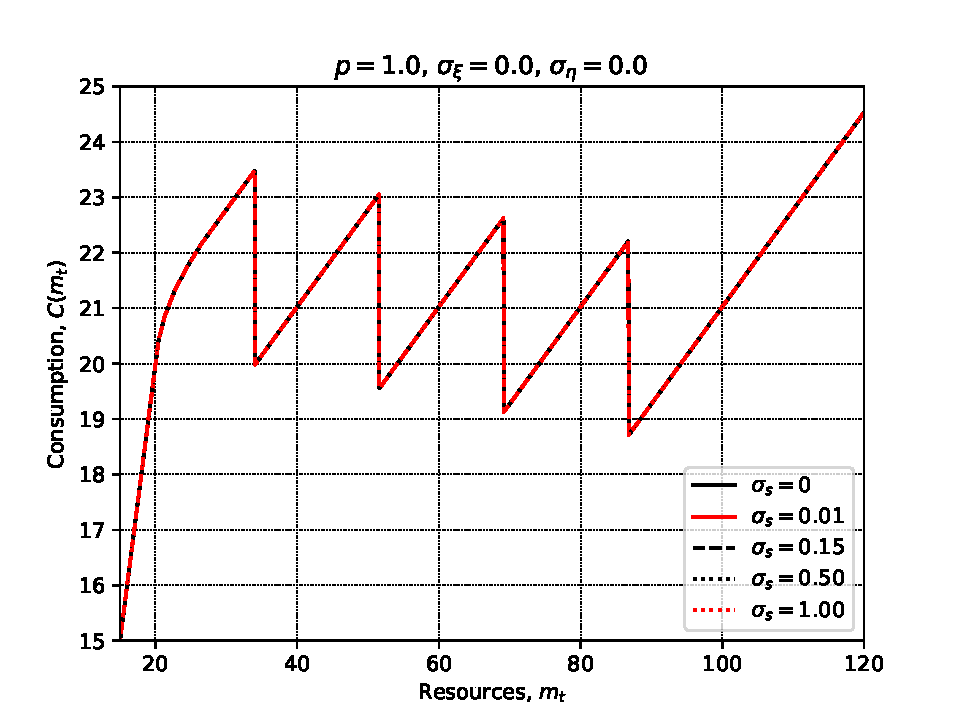
\includegraphics[width=\linewidth]{p1_xi0_eta0.pdf}
    \caption{Have switching option with certainty, $p = 1$.}
\end{subfigure}
\hfill
\begin{subfigure}{0.48\textwidth}
    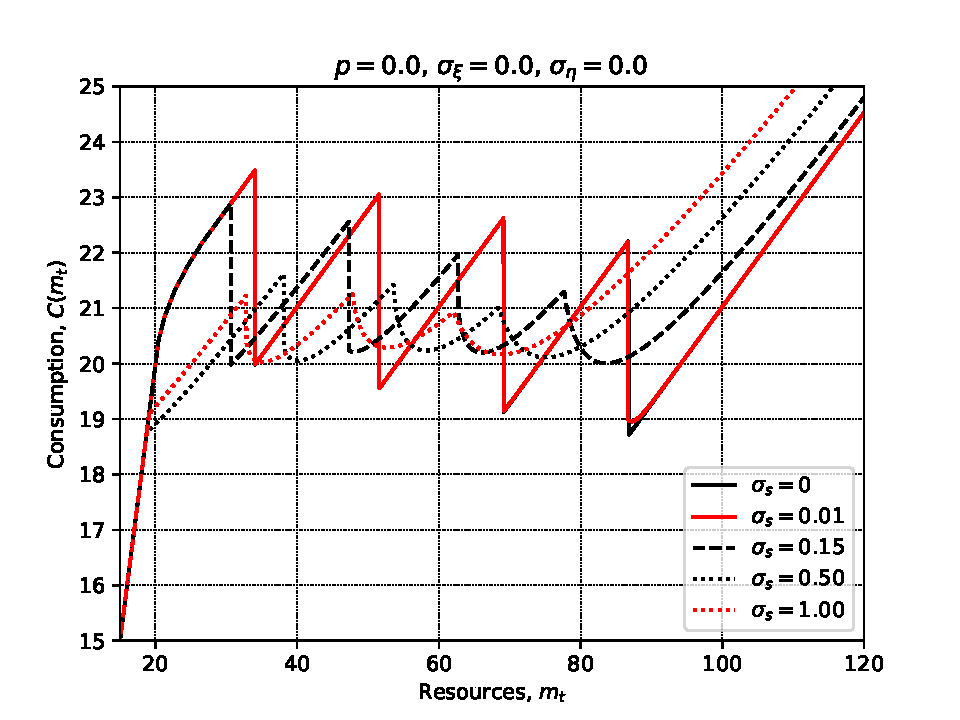
\includegraphics[width=\linewidth]{p0_xi0_eta0.pdf}
    \caption{Stay as worker with certainty without search effort, $p = 0$.}
\end{subfigure}
\caption{The plots show optimal consumption rules of the workers who decides to continue working in period
$t = T - 5$ for a set of search cost scales $\sigma_s$ in the absence of income uncertainty or taste shocks, for the
case with $p = 1.0$ (left panel) with $p = 0.0$ (right panel). The rest of the model parameters are $R = 1$,
$\beta = 0.98$, $y = 20$.}
\label{fig:fig2}
\end{figure}

In contrast, when $p = 0.0$ (Fig.~\ref{fig:fig2}(b)), the worker who does not exert search effort,
continues to stay as a worker with certainty. This gives the worker a motive to exert
search effort, which determines the likelihood of receiving the option to switch. For a
given level of search frictions, decreasing $p$ increases the smoothness of the solution.
Moreover, for a given level of $p$, increasing the search frictions (higher value of $\sigma_s$) also
increases smoothness. Fig.~\ref{fig:fig2}(b) also shows the asymmetric smoothness offered by search,
when there are no taste or income shocks. The smoothness happens to the right of the
discontinuities. This is because for low liquid resources, workers optimally choose to
continue working and hence do not exert any search effort. Workers only exert positive
effort to receive the option to retire when they have ample liquid resources. Therefore,
the smoothness from search frictions only happens to the right of the discontinuities.

To address this asymmetric smoothness, we need to introduce taste shocks. Since
the taste shocks can take a range of different values, there are certain realizations of
the taste shock that make the worker want to have the option to switch, even at levels
of liquid assets at which, in the absence of a taste shock, the worker would not want
to switch. In other words, with the introduction of taste shocks, the range of liquid
assets around the discontinuities over which the worker exerts search effort expands.
Fig.~\ref{fig:fig3}(a) shows that with the incorporation of taste shocks, the consumption function now
smoothes out more uniformly around the discontinuities. Moreover, introducing taste
shocks allows the search frictions to significantly smooths out most of the discontinuities
in the optimal consumption function. This holds even for a very small smoothness
parameter for the taste shocks, $\sigma_\xi = 0.005$. This is because now there is a positive
likelihood of a worker receiving a taste shock that makes them exert search effort even
for values of $M_t$ for which the worker would not exert any search effort in the absence
of taste shocks. Increasing the magnitude of the taste shocks to $\sigma_\xi = 0.02$ (Fig.~\ref{fig:fig3}(b))
significantly reduces the size of all the discontinuities in the consumption function.
Moreover, only moderately sized search frictions are needed to virtually completely
smooth out the consumption function.

%---- Figure 3 ----
\begin{figure}[htbp]
\centering
\begin{subfigure}{0.48\textwidth}
    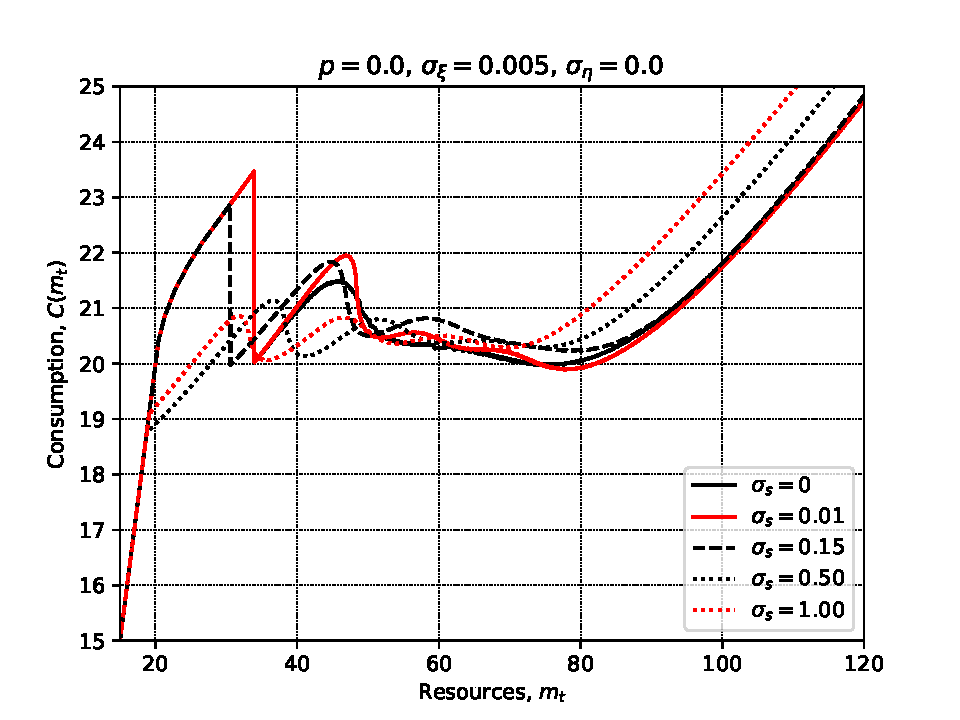
\includegraphics[width=\linewidth]{p0_xi0p005_eta0.pdf}
    \caption{Small taste shocks, $\sigma_\xi = 0.005$.}
\end{subfigure}
\hfill
\begin{subfigure}{0.48\textwidth}
    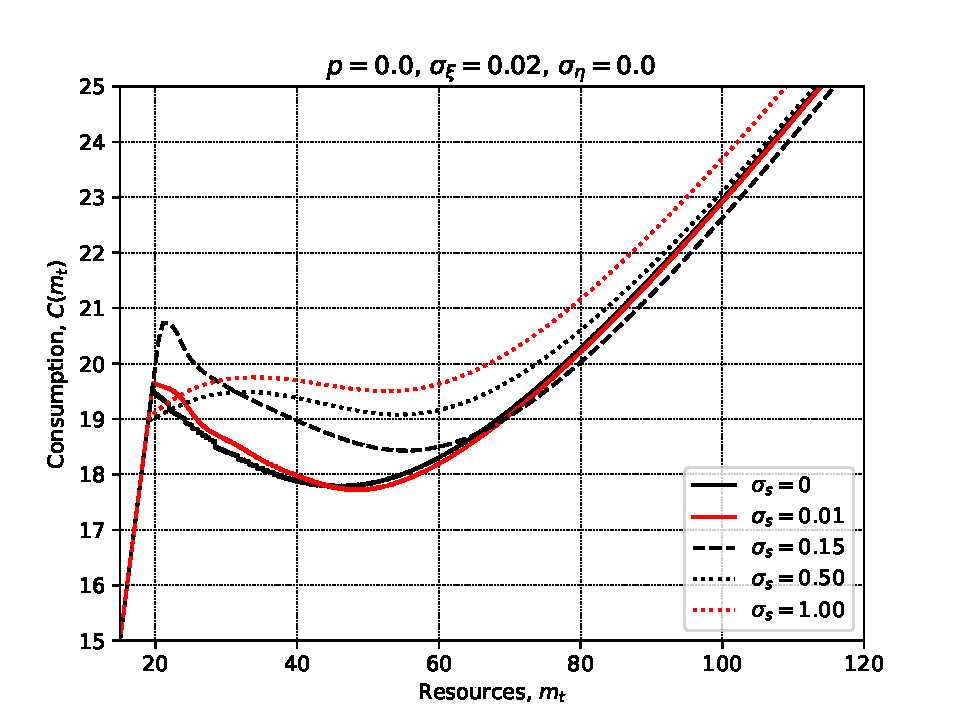
\includegraphics[width=\linewidth]{p0_xi0p02_eta0.pdf}
    \caption{Large taste shocks, $\sigma_\xi = 0.02$.}
\end{subfigure}
\caption{The plots show optimal consumption rules of the workers who decides to continue working in period
$t = T - 5$ for the case with $p = 0$, in the presence of small taste shocks (left panel) and large taste shocks
(right panel), without income uncertainty.}
\label{fig:fig3}
\end{figure}

The results discussed so far do not include any income uncertainty. Adding
income uncertainty even into standard consumption-saving models adds curvature and
smoothness to the consumption rules. We study the impact of incorporating income
uncertainty to the retirement problem on the smoothness of the decision rules in
Figs.~\ref{fig:fig4}(a) and~\ref{fig:fig4}(b). These figures show that while income uncertainty adds smoothness, it does
not play a significant role in reducing the size of the discontinuities. Therefore, search
frictions and taste shocks play the dominant role in smoothing out the problem. An
appropriate combination of search frictions, taste shocks, and income uncertainty can
yield a monotonically increasing outcome-specific consumption function by smoothing
out the discontinuities that propagate through each period while iterating backwards.

%---- Figure 4 ----
\begin{figure}[htbp]
\centering
\begin{subfigure}{0.48\textwidth}
    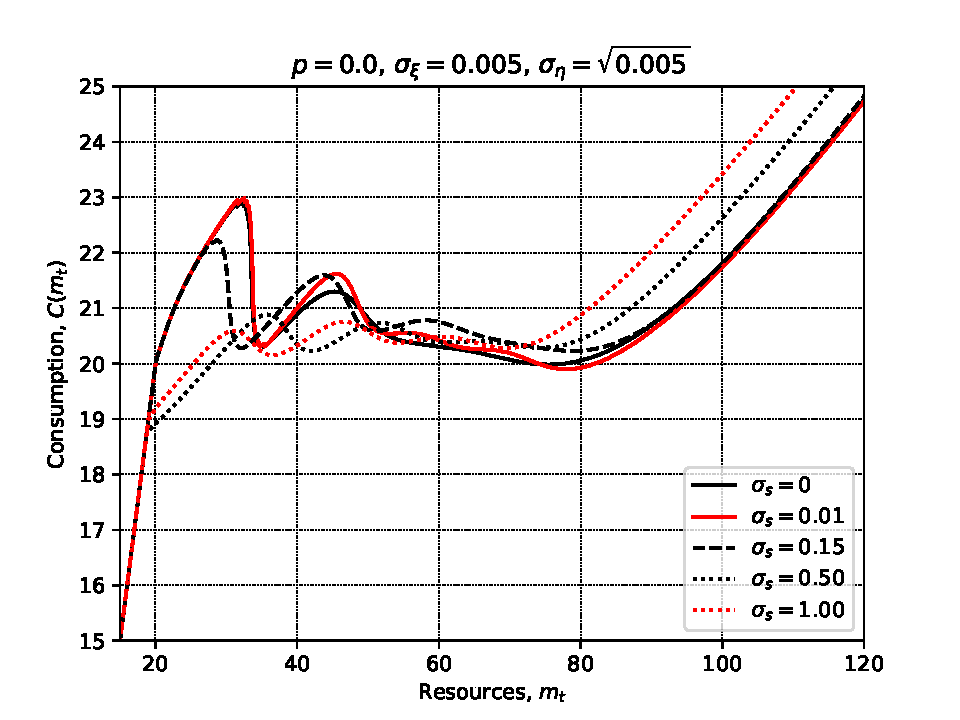
\includegraphics[width=\linewidth]{p0_xi0p005_etaSqrt0p005.pdf}
    \caption{Small taste shocks, $\sigma_\xi = 0.005$.}
\end{subfigure}
\hfill
\begin{subfigure}{0.48\textwidth}
    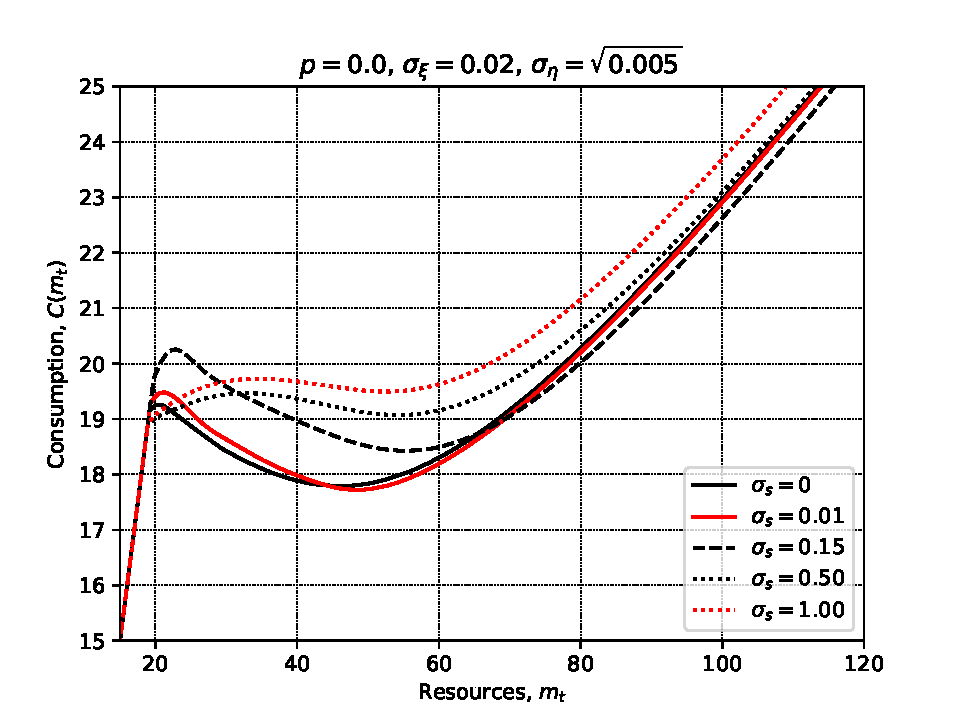
\includegraphics[width=\linewidth]{p0_xi0p02_etaSqrt0p005.pdf}
    \caption{Large taste shocks, $\sigma_\xi = 0.02$.}
\end{subfigure}
\caption{The plots show optimal consumption rules of the workers who decides to continue working in period
$t = T - 5$ for the case with $p = 0$, in the presence of small taste shocks (left panel) and large taste shocks
(right panel), with income uncertainty.}
\label{fig:fig4}
\end{figure}

It is important to note that although each of these smoothness mechanisms serve
to smooth out the solution for the worker's problem, they have different economic
interpretations and affect the optimal consumption rule differently. While lowering
the exogenous probability of receiving the option to switch, $p$, and increasing the search
frictions, $\sigma_s$, shift the consumption function upwards, large taste shocks, $\sigma_\xi$, and income
shocks, $\sigma_\eta$, shift the consumption function downwards. Ceteris paribus, decreasing
$p$ or increasing $\sigma_s$, reduce the likelihood of the worker switching their discrete state
successfully. This means that the likelihood of the worker retiring in a given period
decreases. As a result, the expected number of years that an agent works increases
and they save less in a given period. In contrast, when the size of the taste shocks is
increased, the uncertainty surrounding the likelihood of a worker's retirement decision
increases. Consequently, the agents save more in a given period, because unexpectedly
retiring early would limit the resources that the agent can consume for the remainder of
their life. Similarly, when the size of the income shocks increases, households increase
their buffer stock savings, and the consumption function shifts down. Therefore,
although each of the smoothness mechanisms achieve the common goal of `concavifying'
the solution, they have different interpretations and different impacts on the optimal
consumption rule.

To illustrate these points graphically, we start from the baseline consumption function
that has the discontinuities completely smoothed out using smoothness parameters $p =
0$, $\sigma_\xi = 0.02$, $\sigma_s = 0.5$, and $\sigma_\eta = \sqrt{0.005}$. Fig.~\ref{fig:fig5}(a) shows the impact of lowering $p$ from the
baseline level to $p = 0.1$ and $p = 0.5$, which decreases smoothness, and Fig.~\ref{fig:fig5}(b) shows the
impact of increasing the search frictions from the baseline level to $\sigma_s = 1.0$ and $\sigma_s = 2.0$,
which increases smoothness. As mentioned above, increasing smoothness by adjusting
either of the two mechanisms shifts the optimal consumption rule upwards. On the
other hand, Fig.~\ref{fig:fig6}(a) shows the impact of increasing the size of the taste shocks from the
baseline level to $\sigma_\xi = 0.025$ and $\sigma_\xi = 0.03$, and Fig.~\ref{fig:fig6}(b) shows the impact of increasing the
size of the income shocks from the baseline level to $\sigma_\eta = 5\sqrt{0.005}$ and $\sigma_\eta = 7.5\sqrt{0.005}$.
These figures demonstrate that, as expected, increasing the magnitude of the taste or
income shocks shifts the optimal consumption function downwards. Therefore, while a
combination of these smoothing mechanisms will smooth out the discontinuities, it is
also important to note how each of them shift the decision rule differently.

%---- Figure 5 ----
\begin{figure}[htbp]
\centering
\begin{subfigure}{0.48\textwidth}
    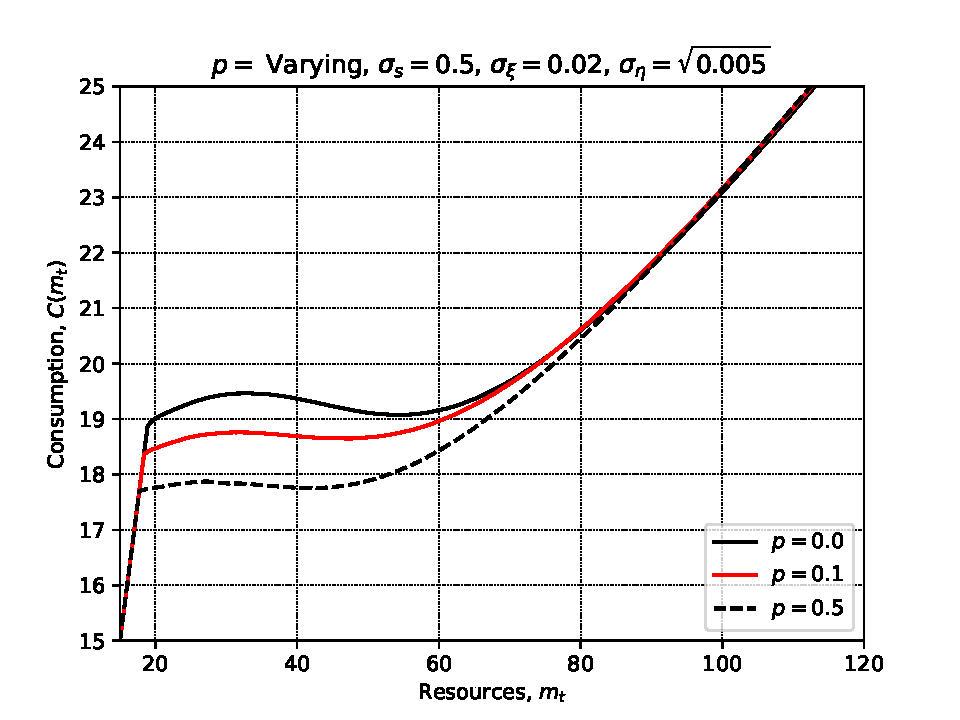
\includegraphics[width=\linewidth]{VaryP.pdf}
    \caption{Varying the exogenous probability of receiving the option to switch.}
\end{subfigure}
\hfill
\begin{subfigure}{0.48\textwidth}
    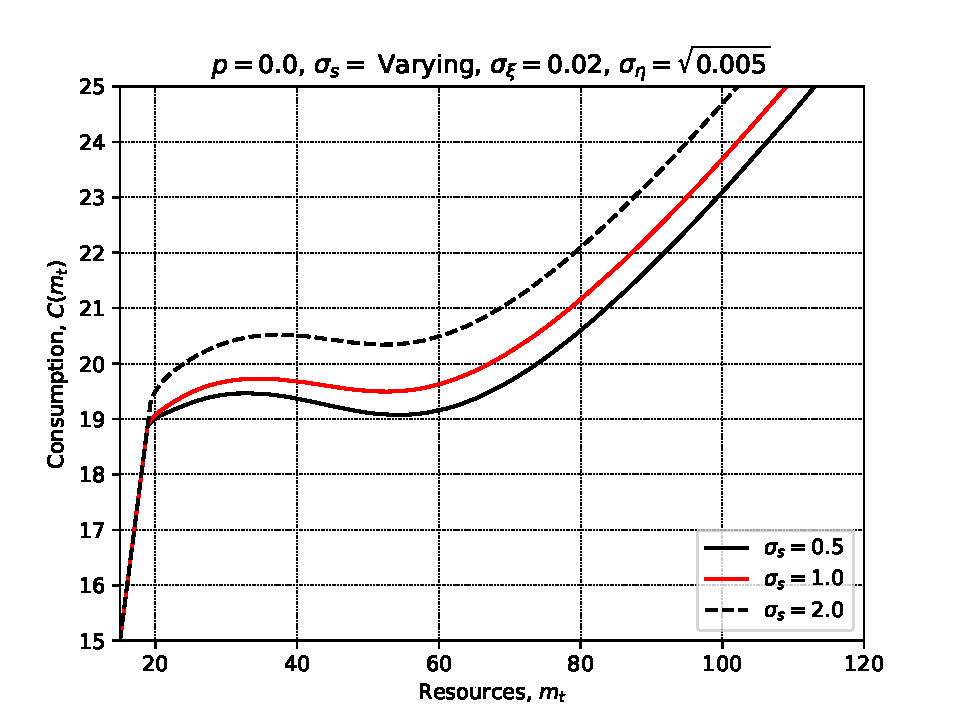
\includegraphics[width=\linewidth]{VaryS.pdf}
    \caption{Varying search friction intensity.}
\end{subfigure}
\caption{The plots show the impact of increasing the smoothness parameters for the exogenous option probability
(left panel) and increasing the magnitude of the search frictions (right panel).}
\label{fig:fig5}
\end{figure}

%---- Figure 6 ----
\begin{figure}[htbp]
\centering
\begin{subfigure}{0.48\textwidth}
    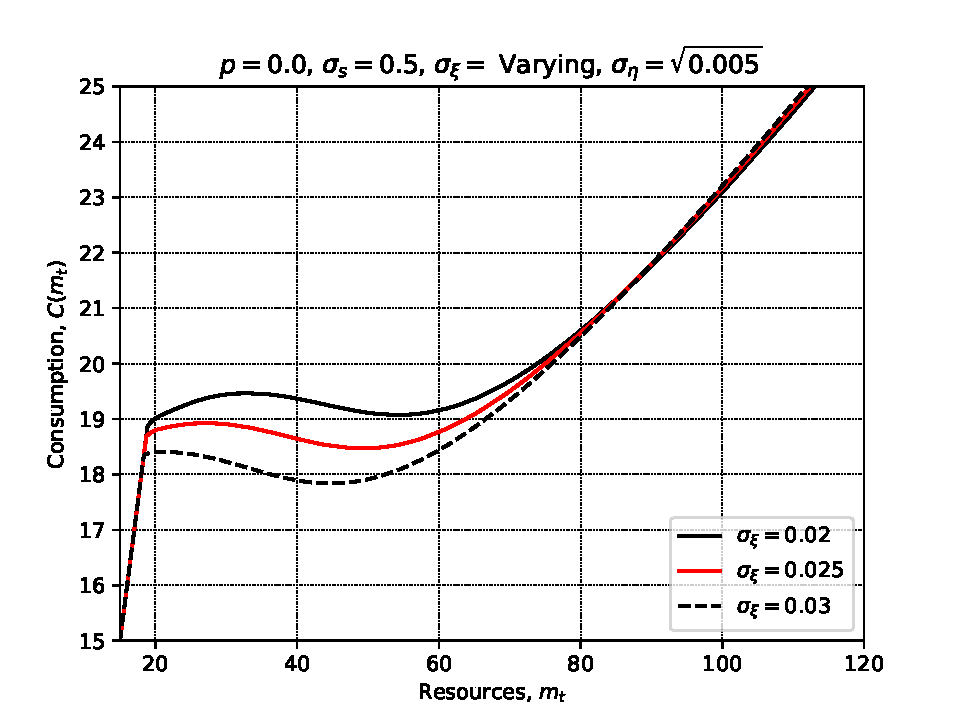
\includegraphics[width=\linewidth]{VaryXi.pdf}
    \caption{Varying the magnitude of the taste shocks.}
\end{subfigure}
\hfill
\begin{subfigure}{0.48\textwidth}
    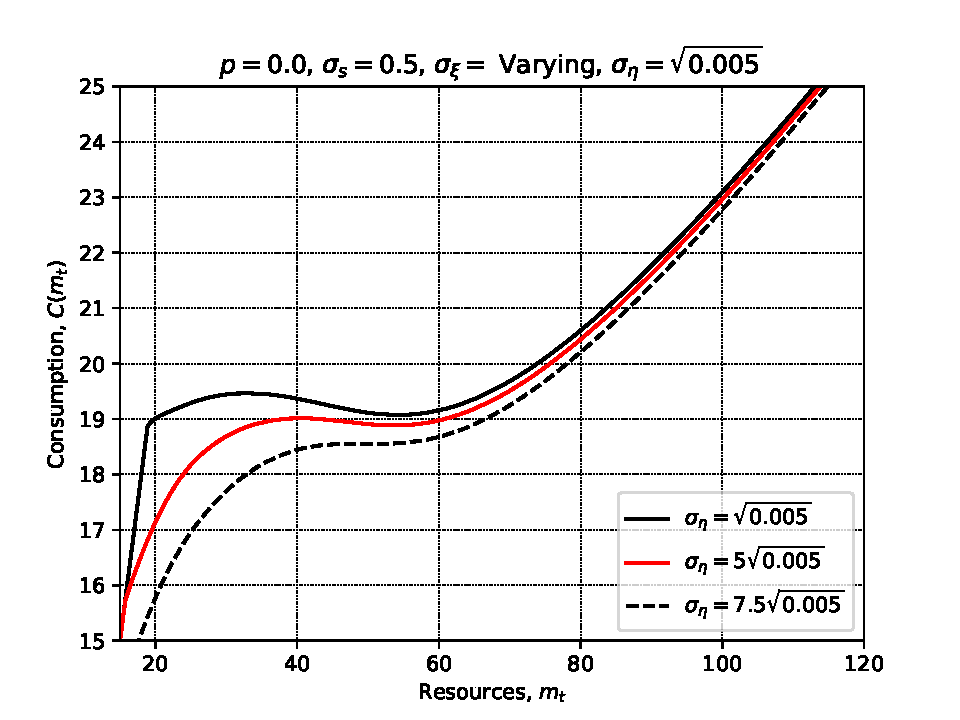
\includegraphics[width=\linewidth]{VaryEta.pdf}
    \caption{Varying the magnitude of the income shocks.}
\end{subfigure}
\caption{The plots show the impact of increasing the smoothness parameters for the taste shocks (left panel) and
increasing the magnitude of the income shocks (right panel).}
\label{fig:fig6}
\end{figure}

%============================================================
\subsection{Income discretization and computational cost}
\label{sec:incdisc}
%============================================================
% STRUCTURE / LAYOUT ONLY --- no numerical results yet.
% (The transition-matrix implementation is under review; the quantitative claims,
%  figure, and timing table below are placeholders to be filled once verified.)

% --- Point being made (numerical vs.\ economic smoothing) ---
The smoothing mechanisms studied above are \emph{economic}: they reshape the agent's
decision rule. This subsection instead isolates a \emph{numerical} source of
non-smoothness that is distinct from, and must not be confused with, the economic
discontinuities generated by the discrete retirement choice. When the continuous income
process is approximated by a coarse discretization, the expected-value and
expected-marginal-utility integrals are computed inaccurately, introducing spurious
kinks into the outcome-specific consumption function. Refining the discretization removes
these artifacts and the solution converges to the true (economically kinked) function.
% [Placeholder: state the headline result once verified --- i.e.\ how many gridpoints
%  are needed for convergence, and how the transition-matrix method compares.]

% --- Experimental design ---
\paragraph{Experiment.}
To isolate the effect of income discretization, we shut down all other smoothing
channels: the option arrives with certainty ($p = 1$), so no search effort is exerted
($\sigma_s = 0$), and there are no taste shocks ($\sigma_\xi = 0$, one taste node). Any
remaining change in the consumption rule is therefore attributable solely to how the
transitory income shock is integrated. Holding the transitory income dispersion
$\sigma_\eta$ fixed, we compare:
\begin{enumerate}
    \item the standard \emph{discretization} of the mean-one lognormal transitory shock,
    with an increasing number of quadrature nodes (e.g.\ $1, 7, 31, 151$ points); and
    \item the \emph{transition-matrix} method (Section~\ref{sec:tranmatrix}), which maps
    end-of-period assets to next-period market resources through a precomputed
    $b \to m$ transition matrix.
\end{enumerate}
We report the outcome-specific consumption rule at $t = T-5$ over a common resource grid.
Model parameters not listed here are $R = 1$, $\beta = 0.98$, $y = 20$.
% [Placeholder: specify the exact \sigma_\eta used in the final figure once chosen.]

% --- Figure placeholder ---
% \begin{figure}[htbp]
% \centering
%     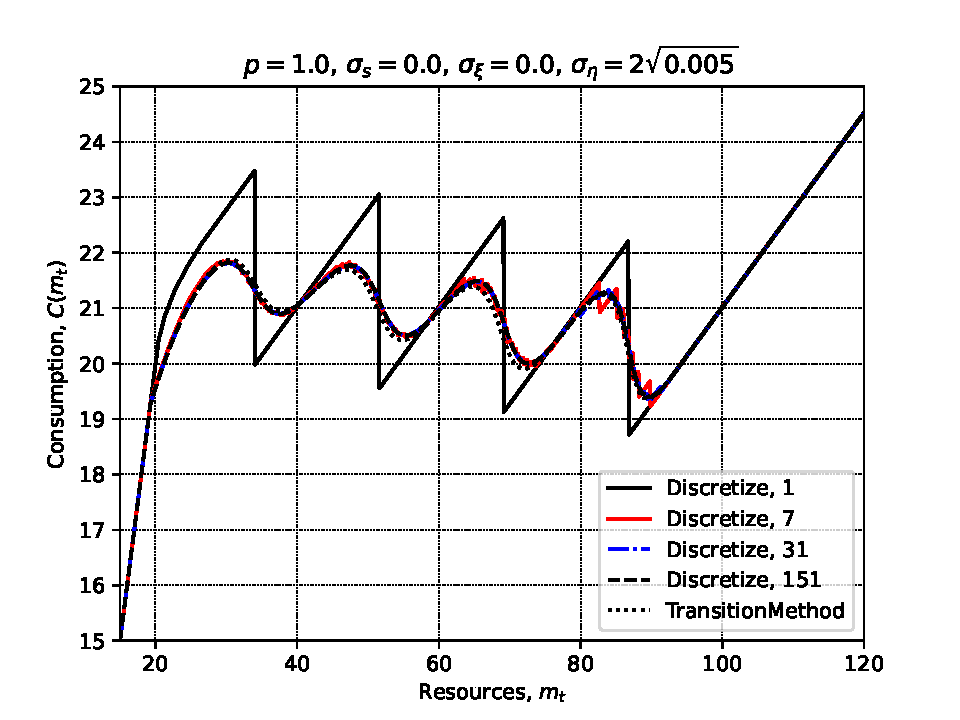
\includegraphics[width=0.6\linewidth]{IncomeDiscMethod_Convergence.pdf}
% \caption{[PLACEHOLDER] Consumption rules under coarse-to-fine income discretization
% and under the transition-matrix method, holding $\sigma_\eta$ fixed
% ($p = 1$, $\sigma_s = 0$, $\sigma_\xi = 0$).}
% \label{fig:incdisc}
% \end{figure}

% --- Accuracy / cost table placeholder ---
\paragraph{Accuracy and cost.}
We assess each method along two dimensions: (i) \emph{accuracy}, measured as the deviation
of its consumption rule from a converged fine-discretization reference; and (ii)
\emph{computational cost}, measured as the solve time. The comparison is summarized in
Table~\ref{tab:incdisc}.
% [Placeholder: fill Table~\ref{tab:incdisc} with verified numbers.]
\begin{table}[htbp]
\centering
\caption{[PLACEHOLDER] Accuracy and solve time by income-integration method.}
\label{tab:incdisc}
\begin{tabular}{lccc}
\toprule
Method & Gridpoints & Solve time (s) & Deviation vs.\ reference \\
\midrule
Discretization    & $1$   & --- & --- \\
Discretization    & $7$   & --- & --- \\
Discretization    & $31$  & --- & --- \\
Discretization    & $151$ & --- & (reference) \\
Transition matrix & ---   & --- & --- \\
\bottomrule
\end{tabular}
\end{table}

% [Placeholder: closing sentence on the accuracy--cost trade-off, to be written once the
%  transition-matrix method is verified.]

%============================================================
\section{Algorithm}
%============================================================
This section outlines the algorithm for solving the problem of the worker who continues
to work in the current period. The problem for the retiree can be pre-solved relatively
easily. With the solution of the worker who continues to work and the retiree at hand,
it is straightforward to compute the solution of the worker with the option to switch.
With ample smoothness, the EGM-step should not produce any suboptimal points.
However, if there is not enough smoothness, then an additional `upper envelope' step
is required to remove the suboptimal points. The upper envelope refinement step in
\citet{ijrs2017} is an example of an algorithm that
can be employed at the end of the EGM-step to achieve this.

\begin{algorithm}[htbp]
\caption{EGM-step with search for the worker who continues to work}
\DontPrintSemicolon
Let $\vec{\eta} = \{\eta_1, \dots, \eta_J\}$ and $\vec{\xi} = \{\xi_1, \dots, \xi_K\}$ be vectors of quadrature points with associated weights
$\vec{\omega} = \{\omega_1, \dots, \omega_J\}$ and $\vec{\mu} = \{\mu_1, \dots, \mu_K\}$, respectively.\;
Form an ascending grid over end-of-period wealth, $\vec{A}_t = \{A_t^1, \dots, A_t^I\}$\;
\For{$i = 1, \dots, I$}{
    \For{$j = 1, \dots, J$}{
        Compute $M_{t+1}^j(A_i) = R A_i + y \eta_{t+1}^j$\;
        \For{$d_{t+1} = 0, 1$}{
            Compute $c_{t+1}^{\Ret}(M_{t+1}^j(A_i))$ by interpolating $c_{t+1}^{\Ret}(\vec{M}_{t+1})$ at the point $M_{t+1}^j(A_i)$\;
            Compute $c_{t+1}^{W}(M_{t+1}^j(A_i))$ by interpolating $c_{t+1}^{W}(\vec{M}_{t+1})$ at the point $M_{t+1}^j(A_i)$\;
            Compute $V_{t+1}^{\Ret}(M_{t+1}^j(A_i))$ by interpolating $V_{t+1}^{\Ret}(\vec{M}_{t+1})$ at the point $M_{t+1}^j(A_i)$\;
            \For{$k = 1, \dots, K$}{
                Compute $V_{t+1}^{W}(M_{t+1}^j(A_i), \xi_k)$ by interpolating $V_{t+1}^{W}(\vec{M}_{t+1})$ at the point $M_{t+1}^j(A_i)$ and multiplying it by $\xi_k$\;
                Compute $V_{t+1}^{RW}(M_{t+1}^j(A_i), \xi_k) = \max\{V_{t+1}^{\Ret}(M_{t+1}^j(A_i)), V_{t+1}^{W}(M_{t+1}^j(A_i), \xi_k)\}$\;
                Compute $\mathbbm{1}_{t+1}^0(M_{t+1}^j(A_i), \xi_k) = 1$ if $V_{t+1}^{\Ret}(M_{t+1}^j(A_i)) \ge V_{t+1}^{W}(M_{t+1}^j(A_i), \xi_k)$ and $0$ otherwise.\;
                Compute $\mathbbm{1}_{t+1}^1(M_{t+1}^j(A_i), \xi_k) = 1 - \mathbbm{1}_{t+1}^0(M_{t+1}^j(A_i), \xi_k)$\;
                Compute $\mathrm{RHS}_1^{\mathrm{pre}}(M_{t+1}^j(A_i), \xi_k) = \mathbbm{1}_{t+1}^0(M_{t+1}^j(A_i), \xi_k) \cdot u'(c_{t+1}^{\Ret}(M_{t+1}^j(A_i))) + \xi_k \cdot \mathbbm{1}_{t+1}^1(M_{t+1}^j(A_i), \xi_k) \cdot u'(c_{t+1}^{W}(M_{t+1}^j(A_i)))$\;
                Compute $\mathrm{RHS}_2^{\mathrm{pre}}(M_{t+1}^j(A_i), \xi_k) = \xi_k \cdot u'(c_{t+1}^{W}(M_{t+1}^j(A_i)))$\;
            }
        }
    }
    Compute $\goth{V}_t^1(A_i) = \sum_{j=1}^{J} \sum_{k=1}^{K} \omega_j \mu_k \cdot V_{t+1}^{RW}(M_{t+1}^j(A_i), \xi_k)$\;
    Compute $\goth{V}_t^2(A_i) = \sum_{j=1}^{J} \sum_{k=1}^{K} \omega_j \mu_k \cdot V_{t+1}^{W}(M_{t+1}^j(A_i), \xi_k)$\;
    Compute $\eff_t(A_i) = 1 - \exp\left(-\beta(1 - p)(\goth{V}_t^1(A_i) - \goth{V}_t^2(A_i))/\sigma_s\right)$\;
    Compute $\theta(\eff_t(A_i)) = \sigma_s (\eff_t(A_i) + (1 - \eff_t(A_i)) \log(1 - \eff_t(A_i)))$\;
    Compute $P_1(\eff_t(A_i)) = (1 - \eff_t(A_i)) \cdot p + \eff_t(A_i)$\;
    Compute $P_2(\eff_t(A_i)) = (1 - \eff_t(A_i)) \cdot (1 - p)$\;
    Compute $\mathrm{RHS}_1(A_i) = \sum_{j=1}^{J} \sum_{k=1}^{K} \omega_j \mu_k \cdot \mathrm{RHS}_1^{\mathrm{pre}}(M_{t+1}^j(A_i), \xi_k)$\;
    Compute $\mathrm{RHS}_2(A_i) = \sum_{j=1}^{J} \sum_{k=1}^{K} \omega_j \mu_k \cdot \mathrm{RHS}_2^{\mathrm{pre}}(M_{t+1}^j(A_i), \xi_k)$\;
    Compute $\mathrm{RHS}(A_i) = R\beta (P_1(\eff_t(A_i)) \mathrm{RHS}_1(A_i) + P_2(\eff_t(A_i)) \mathrm{RHS}_2(A_i))$\;
    Compute expected value function $\E V_{t+1}(M_{t+1}(A_i)) = P_1(\eff_t(A_i)) \cdot \goth{V}_t^1(A_i) + P_2(\eff_t(A_i)) \cdot \goth{V}_t^2(A_i)$\;
    Compute current consumption $c_t^{W}(A_i) = u'^{-1}(\mathrm{RHS}(A_i))$\;
    Compute value function $V_t^{W}(M_t(A_i)) = u(c_t^{W}(A_i), 1, \eff_t(A_i)) + \beta \E V_{t+1}(M_{t+1}(A_i))$\;
    Compute endogenous grid point $M_t(A_i) = c_t^{W}(A_i) + A_i$\;
}
Collect the points $M_t(A_i)$, $c_t^{W}(A_i)$, and $V_t^{W}(M_t(A_i))$ to form the consumption function, $c_t^{W}(\vec{M}_t)$, and value function, $V_t^{W}(\vec{M}_t)$.\;
\end{algorithm}

%------------------------------------------------------------
\subsection{Transition-matrix income integration}
\label{sec:tranmatrix}
%------------------------------------------------------------
% STRUCTURE / METHOD LAYOUT ONLY --- no results or performance claims yet.
% (Implementation under review; see Section~\ref{sec:incdisc} for the experiment.)

In Algorithm~1, the expectation over the transitory income shock is taken by looping over
the $J$ quadrature nodes $\vec{\eta}$ and interpolating the next-period functions at each
implied $M_{t+1}^j(A_i)$. As an alternative, the transitory-income integration can be
recast as a single (precomputed) linear map, following the transition-matrix approach of
\citet{white2015}.

\paragraph{Idea.}
Let $b = R A_t$ denote next-period wealth \emph{before} the income draw, and
$m = R A_t + y\eta$ next-period market resources \emph{after} it. For a fixed income
process, the conditional density of $m$ given $b$ is time-invariant, so the mapping from a
function defined on an $m$-grid to its conditional expectation on a $b$-grid can be encoded
once as a matrix $\Pi$ with entries $\Pi_{b,m} \approx \Pr(m \mid b)$.

\paragraph{Steps.}
\begin{enumerate}
    \item Build dense grids over $b$ and $m$ and construct the transition matrix $\Pi$
    from the (transitory) income density. % [Placeholder: state exact density, grids,
    % and the quadrature/normalization used, once the implementation is verified.]
    \item For each next-period quantity of interest (marginal utility and value), evaluate
    it on the $m$-grid, then obtain its conditional expectation on the $b$-grid by the
    matrix product $\Pi \, f(\vec{m})$.
    \item Interpolate the resulting $b$-grid expectations onto $b = R\,\vec{A}_t$ to replace
    the transitory-shock loop (lines corresponding to the $j$-sum) in Algorithm~1; the
    remaining EGM and envelope steps are unchanged.
\end{enumerate}

\paragraph{Rationale.}
Because $\Pi$ is assembled once and reused across periods and states, the per-period cost of
the income expectation reduces to a matrix multiplication.
% [Placeholder: quantify the accuracy--cost trade-off relative to a fine discretization
%  once the transition-matrix implementation is verified; cross-reference
%  Table~\ref{tab:incdisc} and Figure~\ref{fig:incdisc}.]

%============================================================
\section{Conclusion}
%============================================================
This paper introduces search as a new method for smoothing out discrete-continuous
choice (DC) problems. While search can significantly reduce the size of the disconti-
nuities in the decision rule of a DC problem, to get uniform smoothness around the
discontinuities, we need to incorporate taste shocks as well. Together, search and taste
shocks offer modelers greater control over the degree of smoothness in DC models, while
rationalizing the smoothness into the agent's choice problem. With ample smoothness,
discontinuities in the decision rule can be smoothed out entirely; thus, eliminating the
need for incorporating an additional, computationally costly, step of identifying and
removing suboptimal points generated in the EGM step for DC models. This paper
studies search in the context of a consumption-saving-retirement problem; however, the
framework can be easily applied to models of housing purchase, lumpy firm investments,
and a wide array of other DC models.

% TODO(placeholder, results pending): one-liner on the income-integration method.
% We additionally document how the accuracy of income integration affects the numerical
% smoothness of the decision rule, and describe a transition-matrix method for handling it.
% [State the verified accuracy/cost conclusion here once the implementation is finalized.]

%============================================================
% References
%============================================================
\begin{thebibliography}{9}

\bibitem[Carroll(2006)]{carroll2006}
Carroll, Christopher D. (2006):
``The method of endogenous gridpoints for solving dynamic stochastic optimization problems,''
\textit{Economics Letters}, 91(3), 312--320.

\bibitem[Carroll et al.(2017)]{hark2017}
Carroll, Christopher D., Matthew N. White, and Team Econ-ARK (2017):
``econ-ark/HARK: 0.8.0,''
Available at via doi:10.5281/zenodo.1001068 or at \url{https://doi.org/10.5281/zenodo.1001068}.

\bibitem[Druedahl and J\o rgensen(2017)]{druedahl2017}
Druedahl, Jeppe, and Thomas H\o gholm J\o rgensen (2017):
``A general endogenous grid method for multi-dimensional models with non-convexities and constraints,''
\textit{Journal of Economic Dynamics and Control}, 74, 87--107.

\bibitem[Fella(2014)]{fella2014}
Fella, Giulio (2014):
``A generalized endogenous grid method for non-smooth and non-concave problems,''
\textit{Review of Economic Dynamics}, 17(2), 329--344.

\bibitem[Iskhakov et al.(2017)]{ijrs2017}
Iskhakov, Fedor, Thomas H. J\o rgensen, John Rust, and Bertel Schjerning (2017):
``The endogenous grid method for discrete-continuous dynamic choice models with (or without) taste shocks,''
\textit{Quantitative Economics}, 8(2), 317--365.

\bibitem[McFadden(1973)]{mcfadden1973}
McFadden, Daniel (1973):
``Conditional logit analysis of qualitative choice behavior,''
in \textit{Frontiers in econometrics}, ed.\ by P. Zarembka, Academic Press, New York.

\bibitem[White(2015)]{white2015}
White, Matthew N. (2015):
``The method of endogenous gridpoints in theory and practice,''
\textit{Journal of Economic Dynamics and Control}, 60, 26--41.

\end{thebibliography}

\end{document}
